
\documentclass{article}
\usepackage{graphicx} % Required for inserting images
\usepackage[spanish]{babel}
\usepackage{charter}
\usepackage{booktabs}
\usepackage[left=1in,right=1in,top=1in,bottom=1in]{geometry}
%\setlength{\parindent}{0pt}
\setlength{\parskip}{0.6em}
\title{Reporte de Estado de la Biodiversidad de Bogotá}
\date{Diciembre 2025}
\author{Carlos Vargas y Nelson Salinas (eds.)}
\begin{document}

\maketitle

\section*{Coberturas}

\noindent \textbf{\large Hernán Serrano}

\noindent \emph{Jardín Botánico de Bogotá, eje Conservación \emph{in situ}}

\bigskip

			
El estudio de las coberturas de la tierra y los ecosistemas es esencial para comprender la dinámica territorial y garantizar una planificación urbana sostenible. Las coberturas actuales representan el uso que el ser humano le da al territorio, mientras que el estudio de los ecosistemas de referencia revela el potencial natural y la vocación de la tierra. La comparación entre ambos es útil para:
			
- Cuantificar la pérdida de biodiversidad y la degradación de hábitats.

- Evaluar la presión antrópica sobre recursos vitales (como el agua y el suelo).

- Identificar áreas prioritarias para la conservación y la restauración ecológica, asegurando que las intervenciones estén dirigidas a reconstruir el Ecosistema Potencial de Referencia (EPR).

Para el territorio de Bogotá, D. C., esta información es vital para la gestión del riesgo y la toma de decisiones relativas a la Estructura Ecológica Principal (EEP), especialmente en zonas de alta fragilidad como el páramo y el bosque altoandino. Para ello se delimitaron espacialmente los diferentes ecosistemas utilizando la base cartográfica del Mapa de Ecosistemas Continentales, Costeros y Marinos (MEC) a escala 1:100.000 (IDEAM 2024). De esta manera se identificaron 12 ecosistemas, entre los que destacan los páramos (55\%) y los bosques (15\%), que ocupan un 70\% del territorio. Por otro lado, los territorios artificializados (IDEAM 2024) cubren cerca del 21\% del área de la ciudad. 

El área correspondiente a ecosistemas transformados, asociados a procesos de intervención (principalmente producción agropecuaria y expansión urbana), fue reconstruida a su Ecosistema Potencial de Referencia (EPR). Los resultados indican que el 70\% de las áreas transformadas correspondían a páramos y bosques altoandinos en el pasado, y que más de la mitad de los ecosistemas originales de Bogotá han desaparecido o están transformados en áreas urbanas y agroecosistemas. De esta manera, los ecosistemas con mayor transformación son humedales (88\%), bosques (81\%), enclaves subxerofíticos (77\%) y páramos (50\%).

Que el 70\% de nuestras áreas impactadas tengan el potencial de volver a ser páramo o bosque altoandino no es solo una cifra, es una oportunidad tangible y urgente. La mitad de nuestros ecosistemas originales esperan nuestra acción. Proteger lo que queda y trabajar decididamente para restaurar el potencial natural de estas áreas no es solo una meta ambiental, sino una inversión directa en la calidad del aire, el suministro de agua y la seguridad frente a los riesgos. El momento de actuar es ahora y requiere el compromiso colectivo de cada ciudadano para garantizar la sostenibilidad y el bienestar de las próximas generaciones.


\bigskip

\begin{figure}[b]
\centering
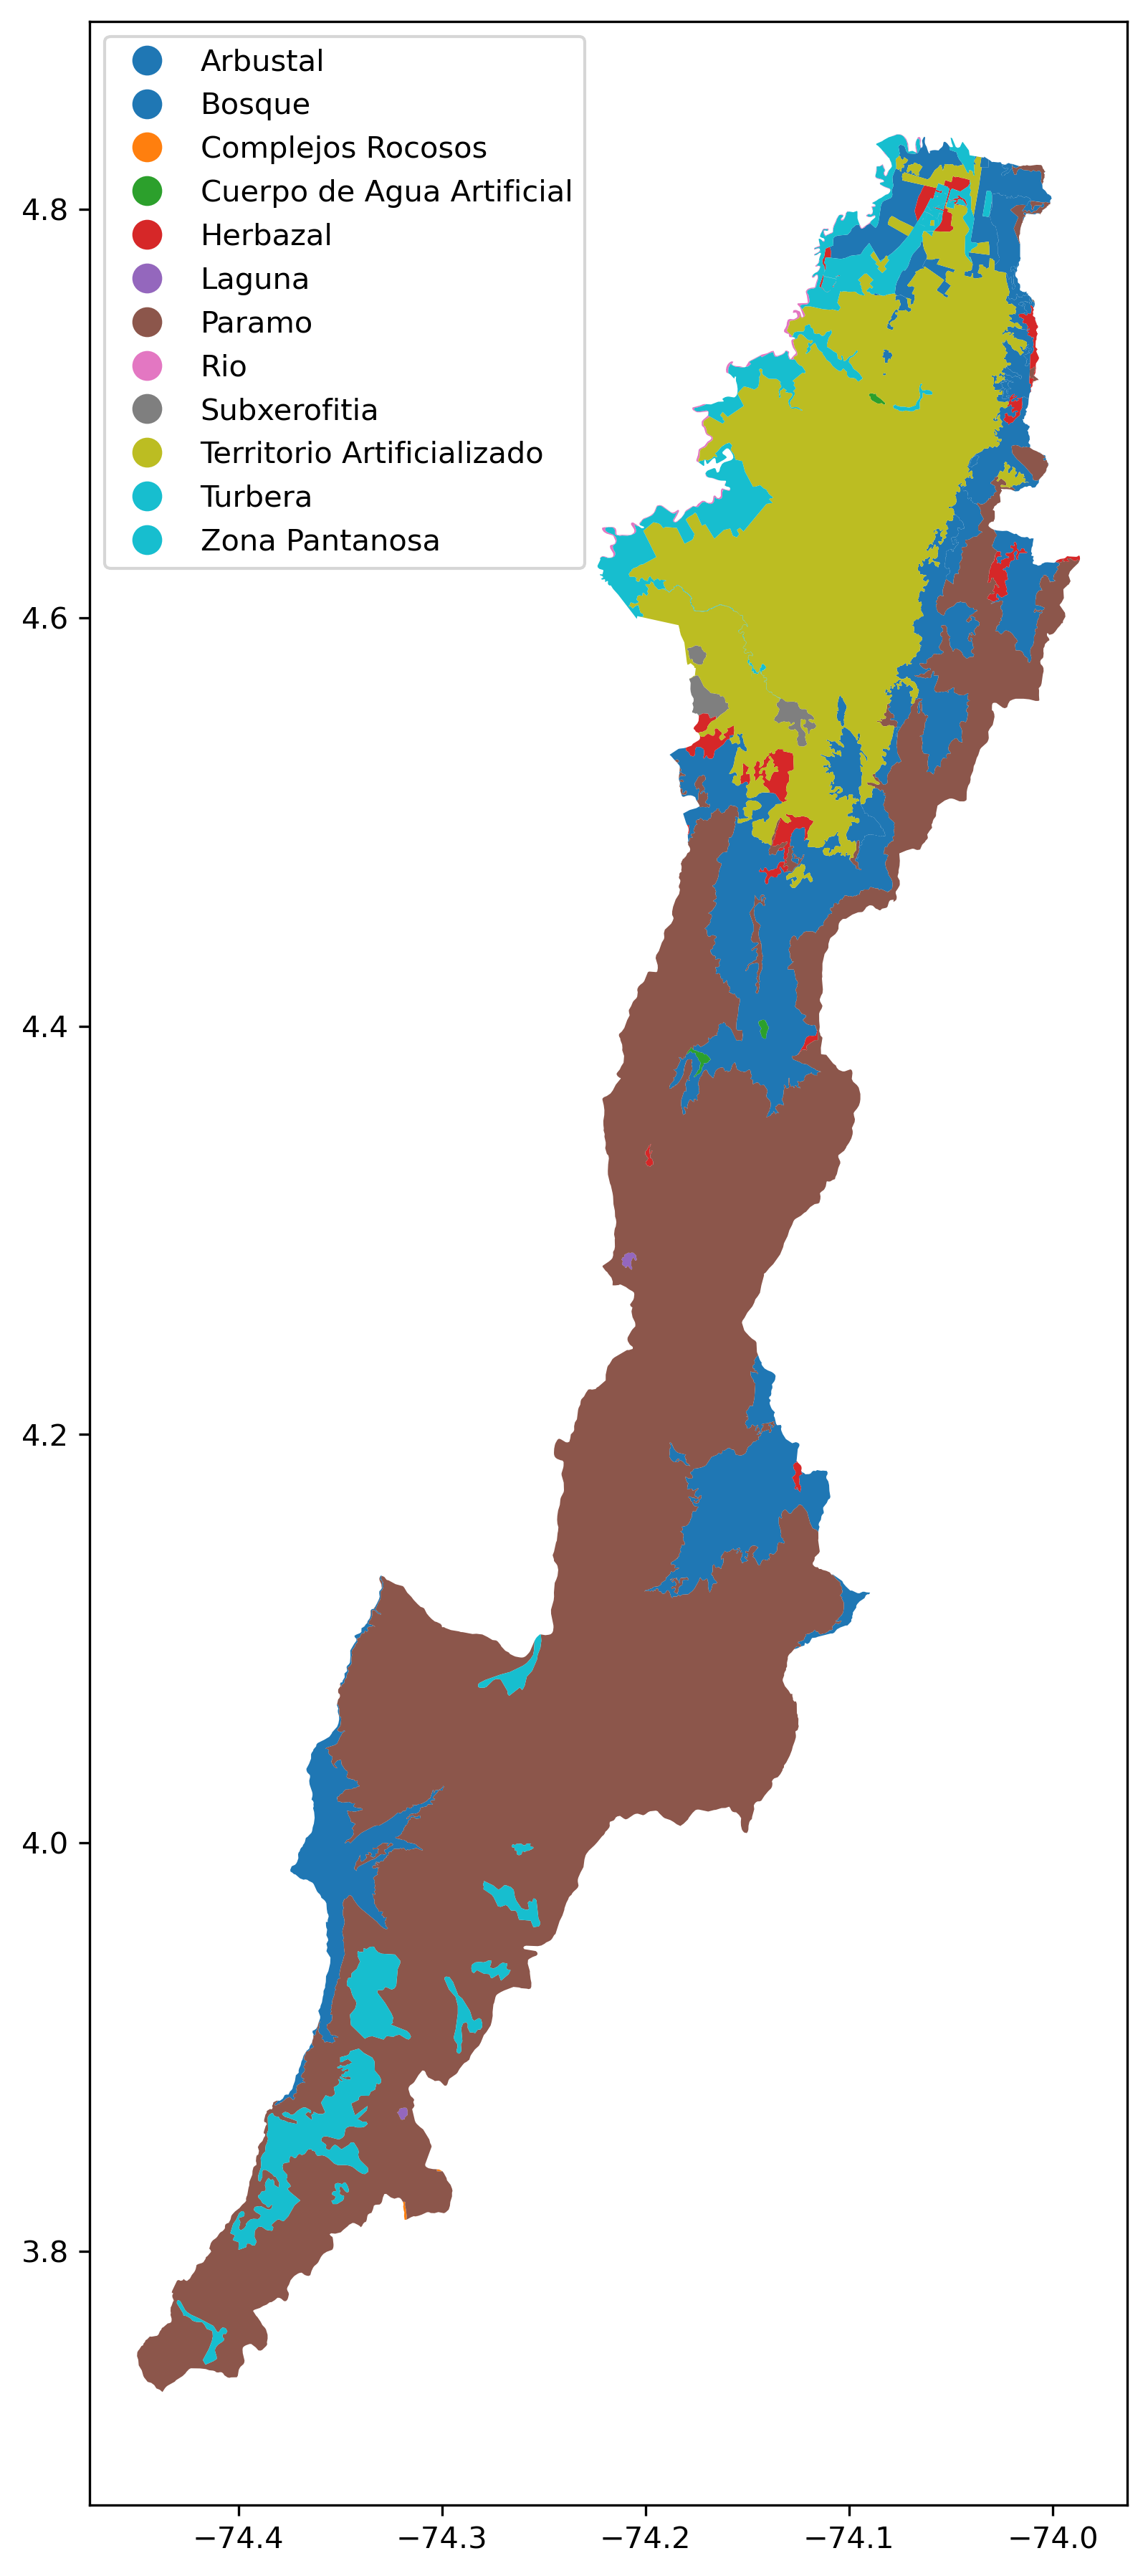
\includegraphics[height=0.8\textheight]{1_coberturas/fig_1.png}
\caption{Coberturas vegetales originales.}
\label{1_coberturas_fig_1}
\end{figure}

\begin{figure}[b]
\centering
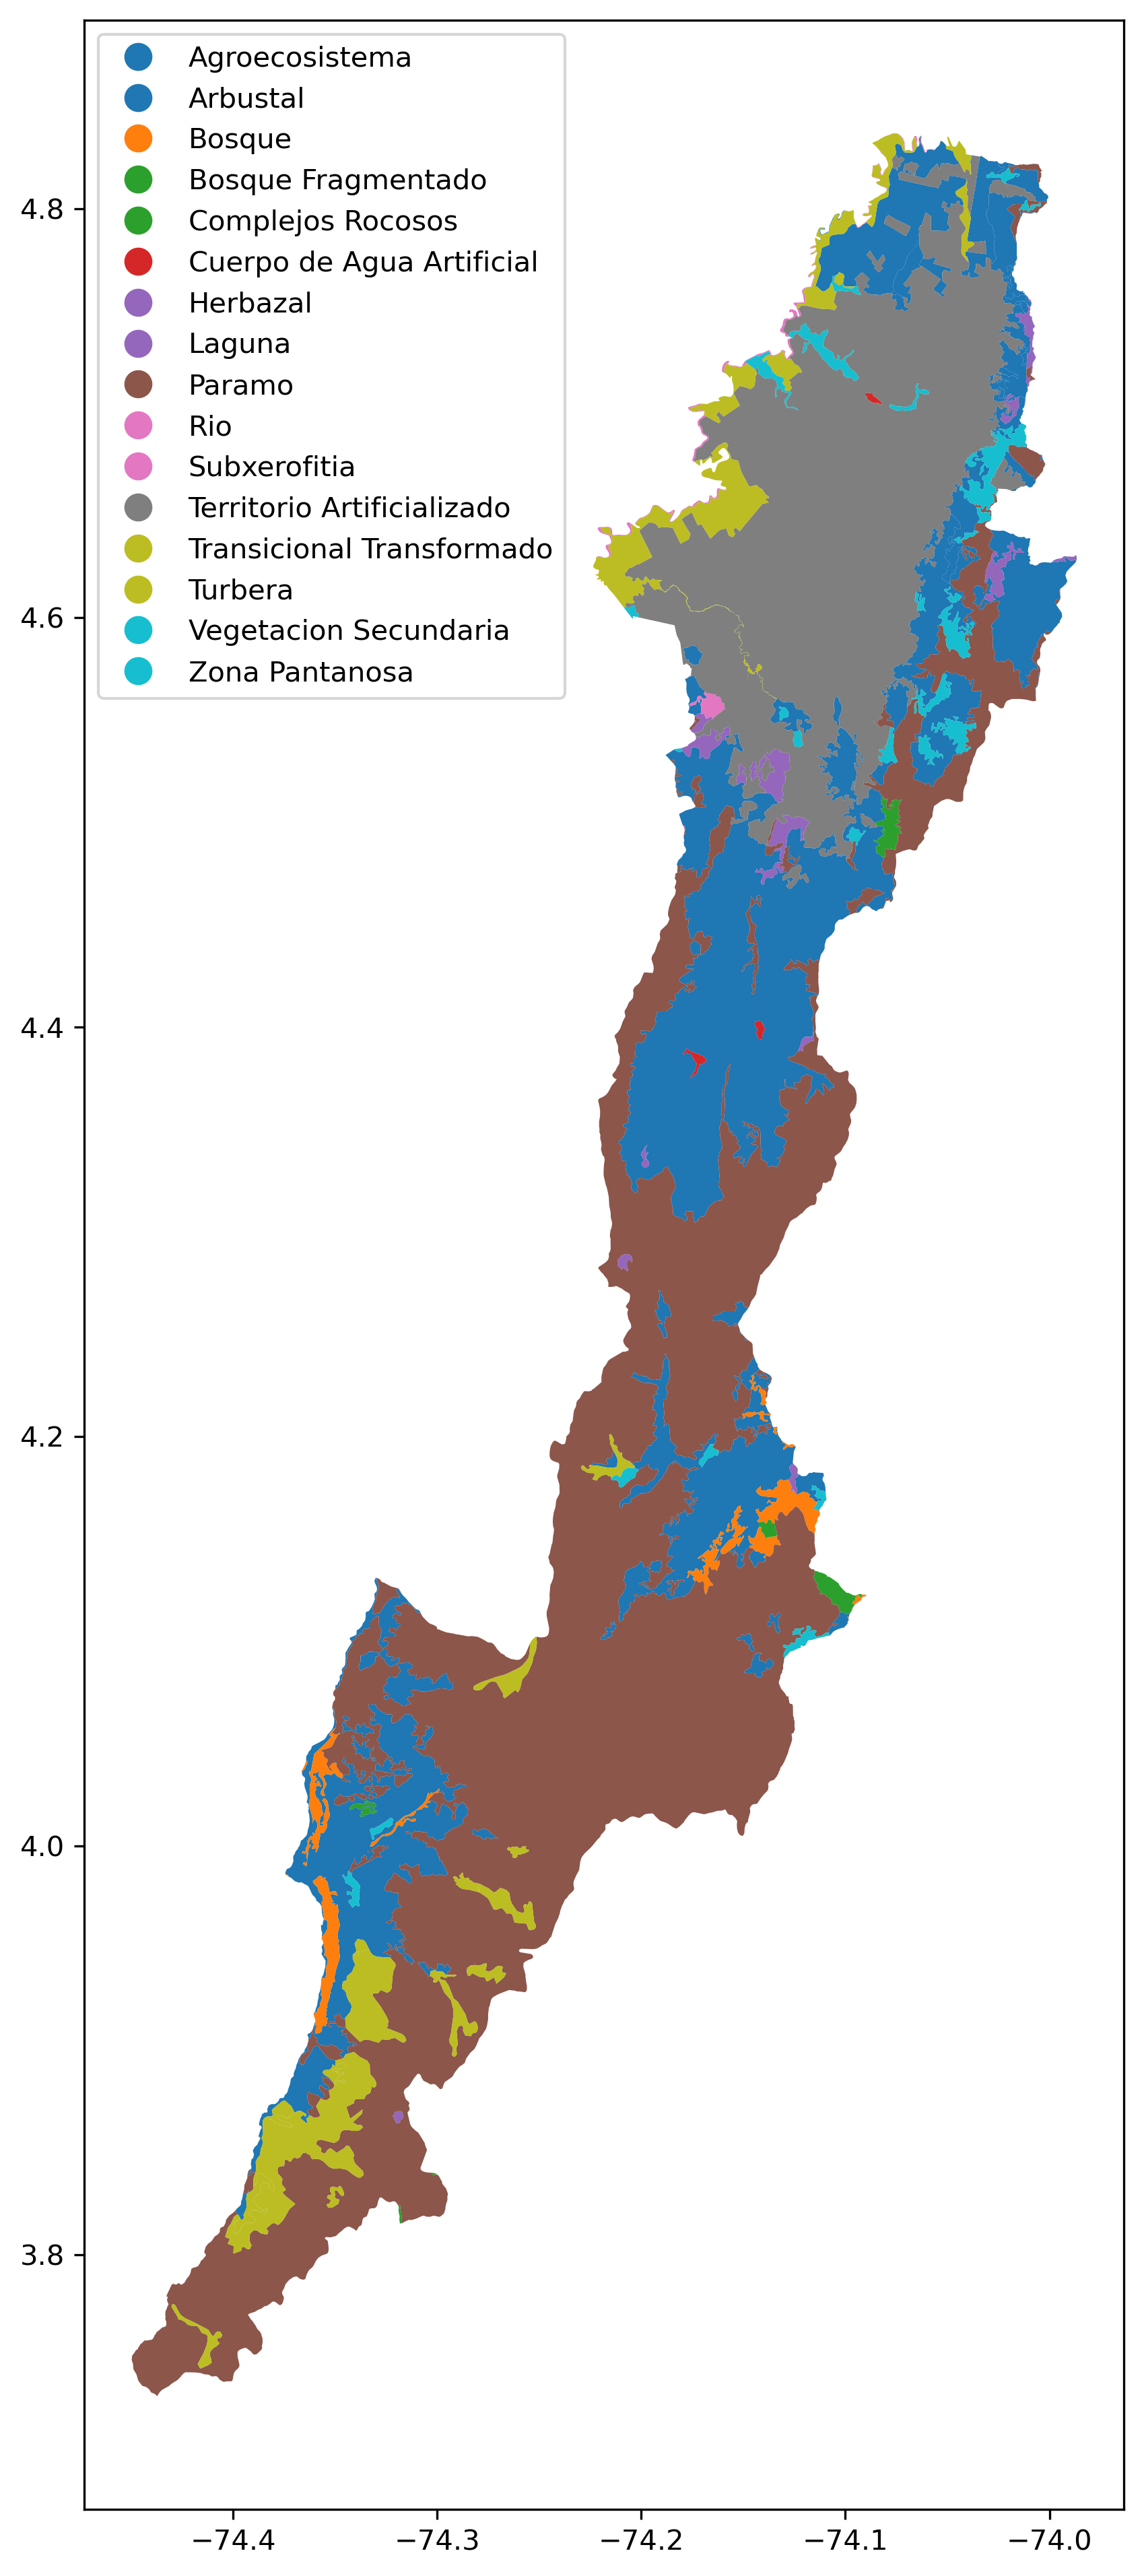
\includegraphics[height=0.8\textheight]{1_coberturas/fig_2.png}
\caption{Coberturas vegetales actuales.}
\label{1_coberturas_fig_2}
\end{figure}

\clearpage

\newpage

\section*{Conectividad de las áreas verdes de Bogotá}

\noindent \textbf{\large Kristian Rubiano}

\noindent \emph{Jardín Botánico de Bogotá, eje Conservación \emph{in situ}}

\bigskip

			
Bogotá se ubica en una de las regiones más biodiversas del planeta, pero su rápido crecimiento urbano ha fragmentado y aislado muchas de sus áreas verdes. Para mitigar estos procesos que impactan negativamente a la biodiversidad, se creó la Estructura Ecológica Principal de Bogotá: una red de cerros, reservas, humedales, rondas de río, parques urbanos y otras áreas verdes, diseñada para conservar la naturaleza y los servicios que esta le presta a ciudad y a la región. Sin embargo, hasta ahora no se sabía con claridad qué tan bien conectados están estos espacios entre sí para proteger la biodiversidad de forma efectiva. 
			
Para ampliar nuestro conocimiento al respecto, usamos mapas detallados de la Estructura Ecológica Principal para analizar cómo están distribuidas estas áreas verdes y qué tan fácil sería para animales como aves, insectos o pequeños mamíferos desplazarse entre ellas, teniendo en cuenta las distancias entre los distintos espacios. Esto también nos permitió identificar zonas de la región que podrían ser priorizadas para aumentar la conectividad entre áreas verdes.
			
Estos análisis indicaron que cerca del 93\% del área de la Estructura Ecológica Principal forma un gran “bloque” continuo de hábitat, lo que es una buena noticia para muchas especies. No obstante, dentro de la ciudad existen zonas, sobre todo altamente urbanizadas y localizadas en el borde sur, donde la Estructura Ecológica Principal casi no está presente y, por lo tanto, la conectividad es muy baja o nula. Estas zonas aparecen como "vacíos" de conectividad y deberían ser prioridad para aumentar y mejorar la presencia y calidad de las áreas verdes.
			
Los parques urbanos de menor tamaño agregan poca área verde adicional al total de la ciudad, pero cumplen un papel clave como pequeños puentes entre las grandes áreas verdes. Disminuyen las distancias entre áreas, aumentan la proximidad entre ellas y refuerzan la posibilidad de movimiento de la fauna a través de la ciudad. Es decir, aunque no sean grandes reservas de hábitat, ayudan a conectar las que ya existen y a llevar la naturaleza a barrios donde hoy casi no hay.
			
En conjunto, los resultados muestran que la Estructura Ecológica Principal ofrece una base sólida de hábitat, mientras que los parques urbanos de menor tamaño ayudan a tejer la red de conexiones entre esos núcleos principales. Esto sugiere que, si se diseñan y manejan con criterios ecológicos (tipo de vegetación, función, tamaño y ubicación), estos parques pueden convertirse en aliados estratégicos para conservar la biodiversidad y mejorar la calidad de vida en Bogotá. Por ello, deberían ser considerados de manera explícita en la planificación y en el seguimiento de cómo se conectan las áreas verdes en la ciudad.


\bigskip

\begin{figure}[b]
\centering

\includegraphics[width=0.7\textwidth]{2_conectividad/fig_1.pdf}
\caption{Conectividad de la estructura ecológica principal.}
\label{2_conectividad_fig_1}
\end{figure}

\begin{figure}[b]
\centering

\includegraphics[width=0.7\textwidth]{2_conectividad/fig_2.pdf}
\caption{Conectividad de la estructura ecológica principal y los parques urbanos.}
\label{2_conectividad_fig_2}
\end{figure}

\begin{figure}[b]
\centering
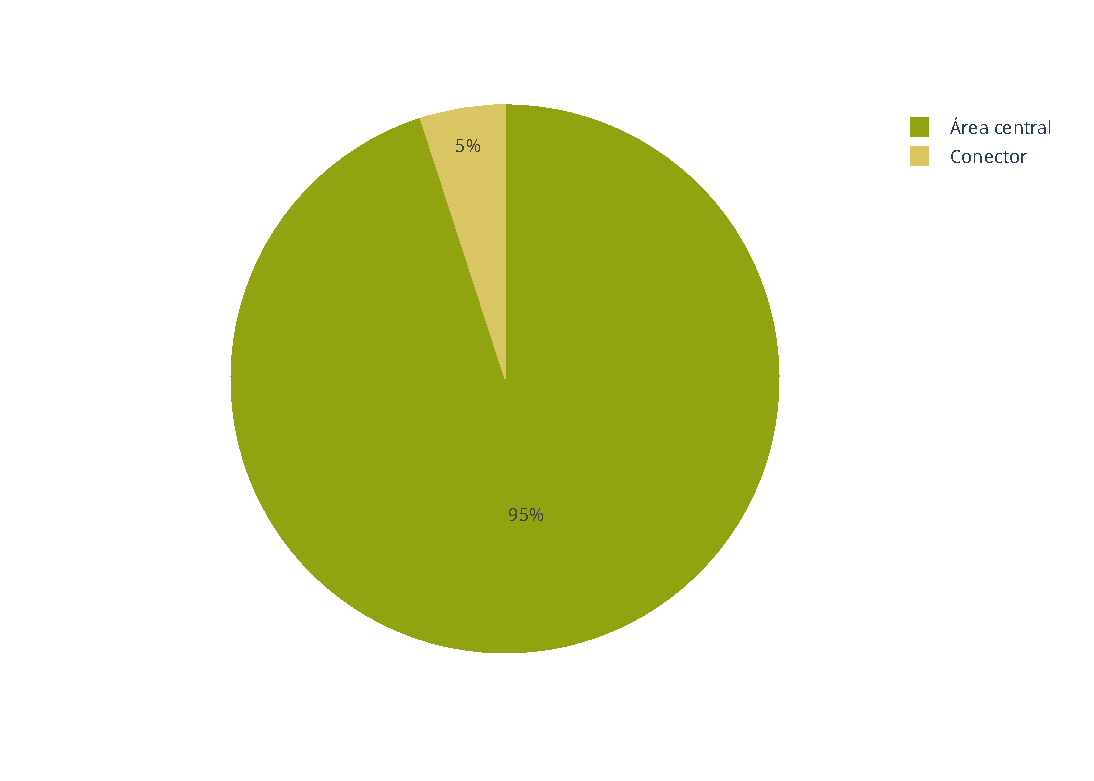
\includegraphics[width=0.7\textwidth]{2_conectividad/fig_3.pdf}
\caption{Tipo de área de la estructura ecológica principal.}
\label{2_conectividad_fig_3}
\end{figure}

\begin{figure}[b]
\centering
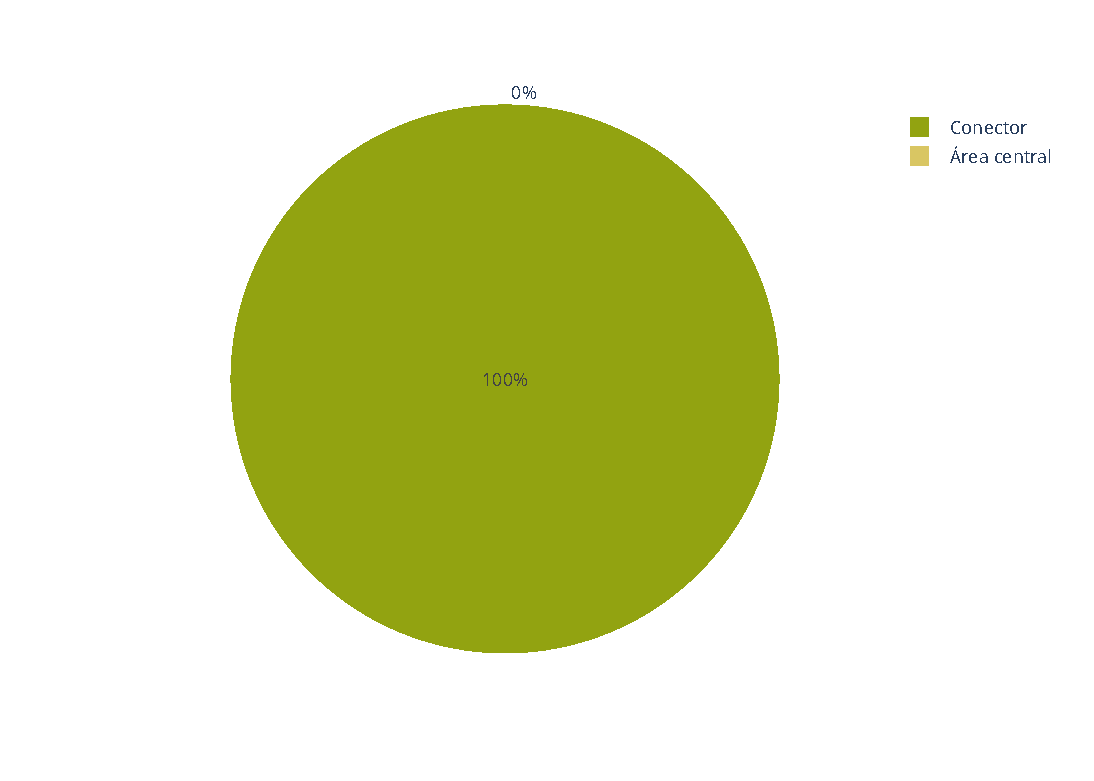
\includegraphics[width=0.7\textwidth]{2_conectividad/fig_4.pdf}
\caption{Tipo de área de los parques urbanos.}
\label{2_conectividad_fig_4}
\end{figure}

\begin{figure}[b]
\centering
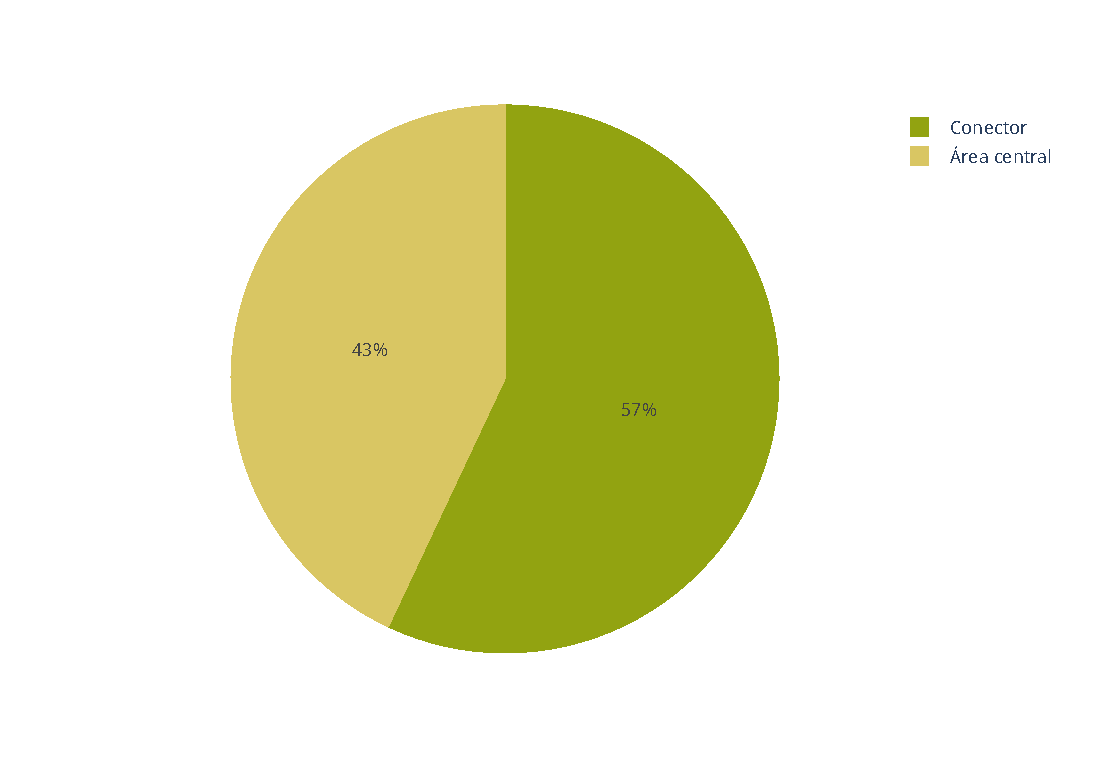
\includegraphics[width=0.7\textwidth]{2_conectividad/fig_5.pdf}
\caption{Tipo de área de las estructura ecológica principal y los parques urbanos.}
\label{2_conectividad_fig_5}
\end{figure}

\begin{figure}[b]
\centering
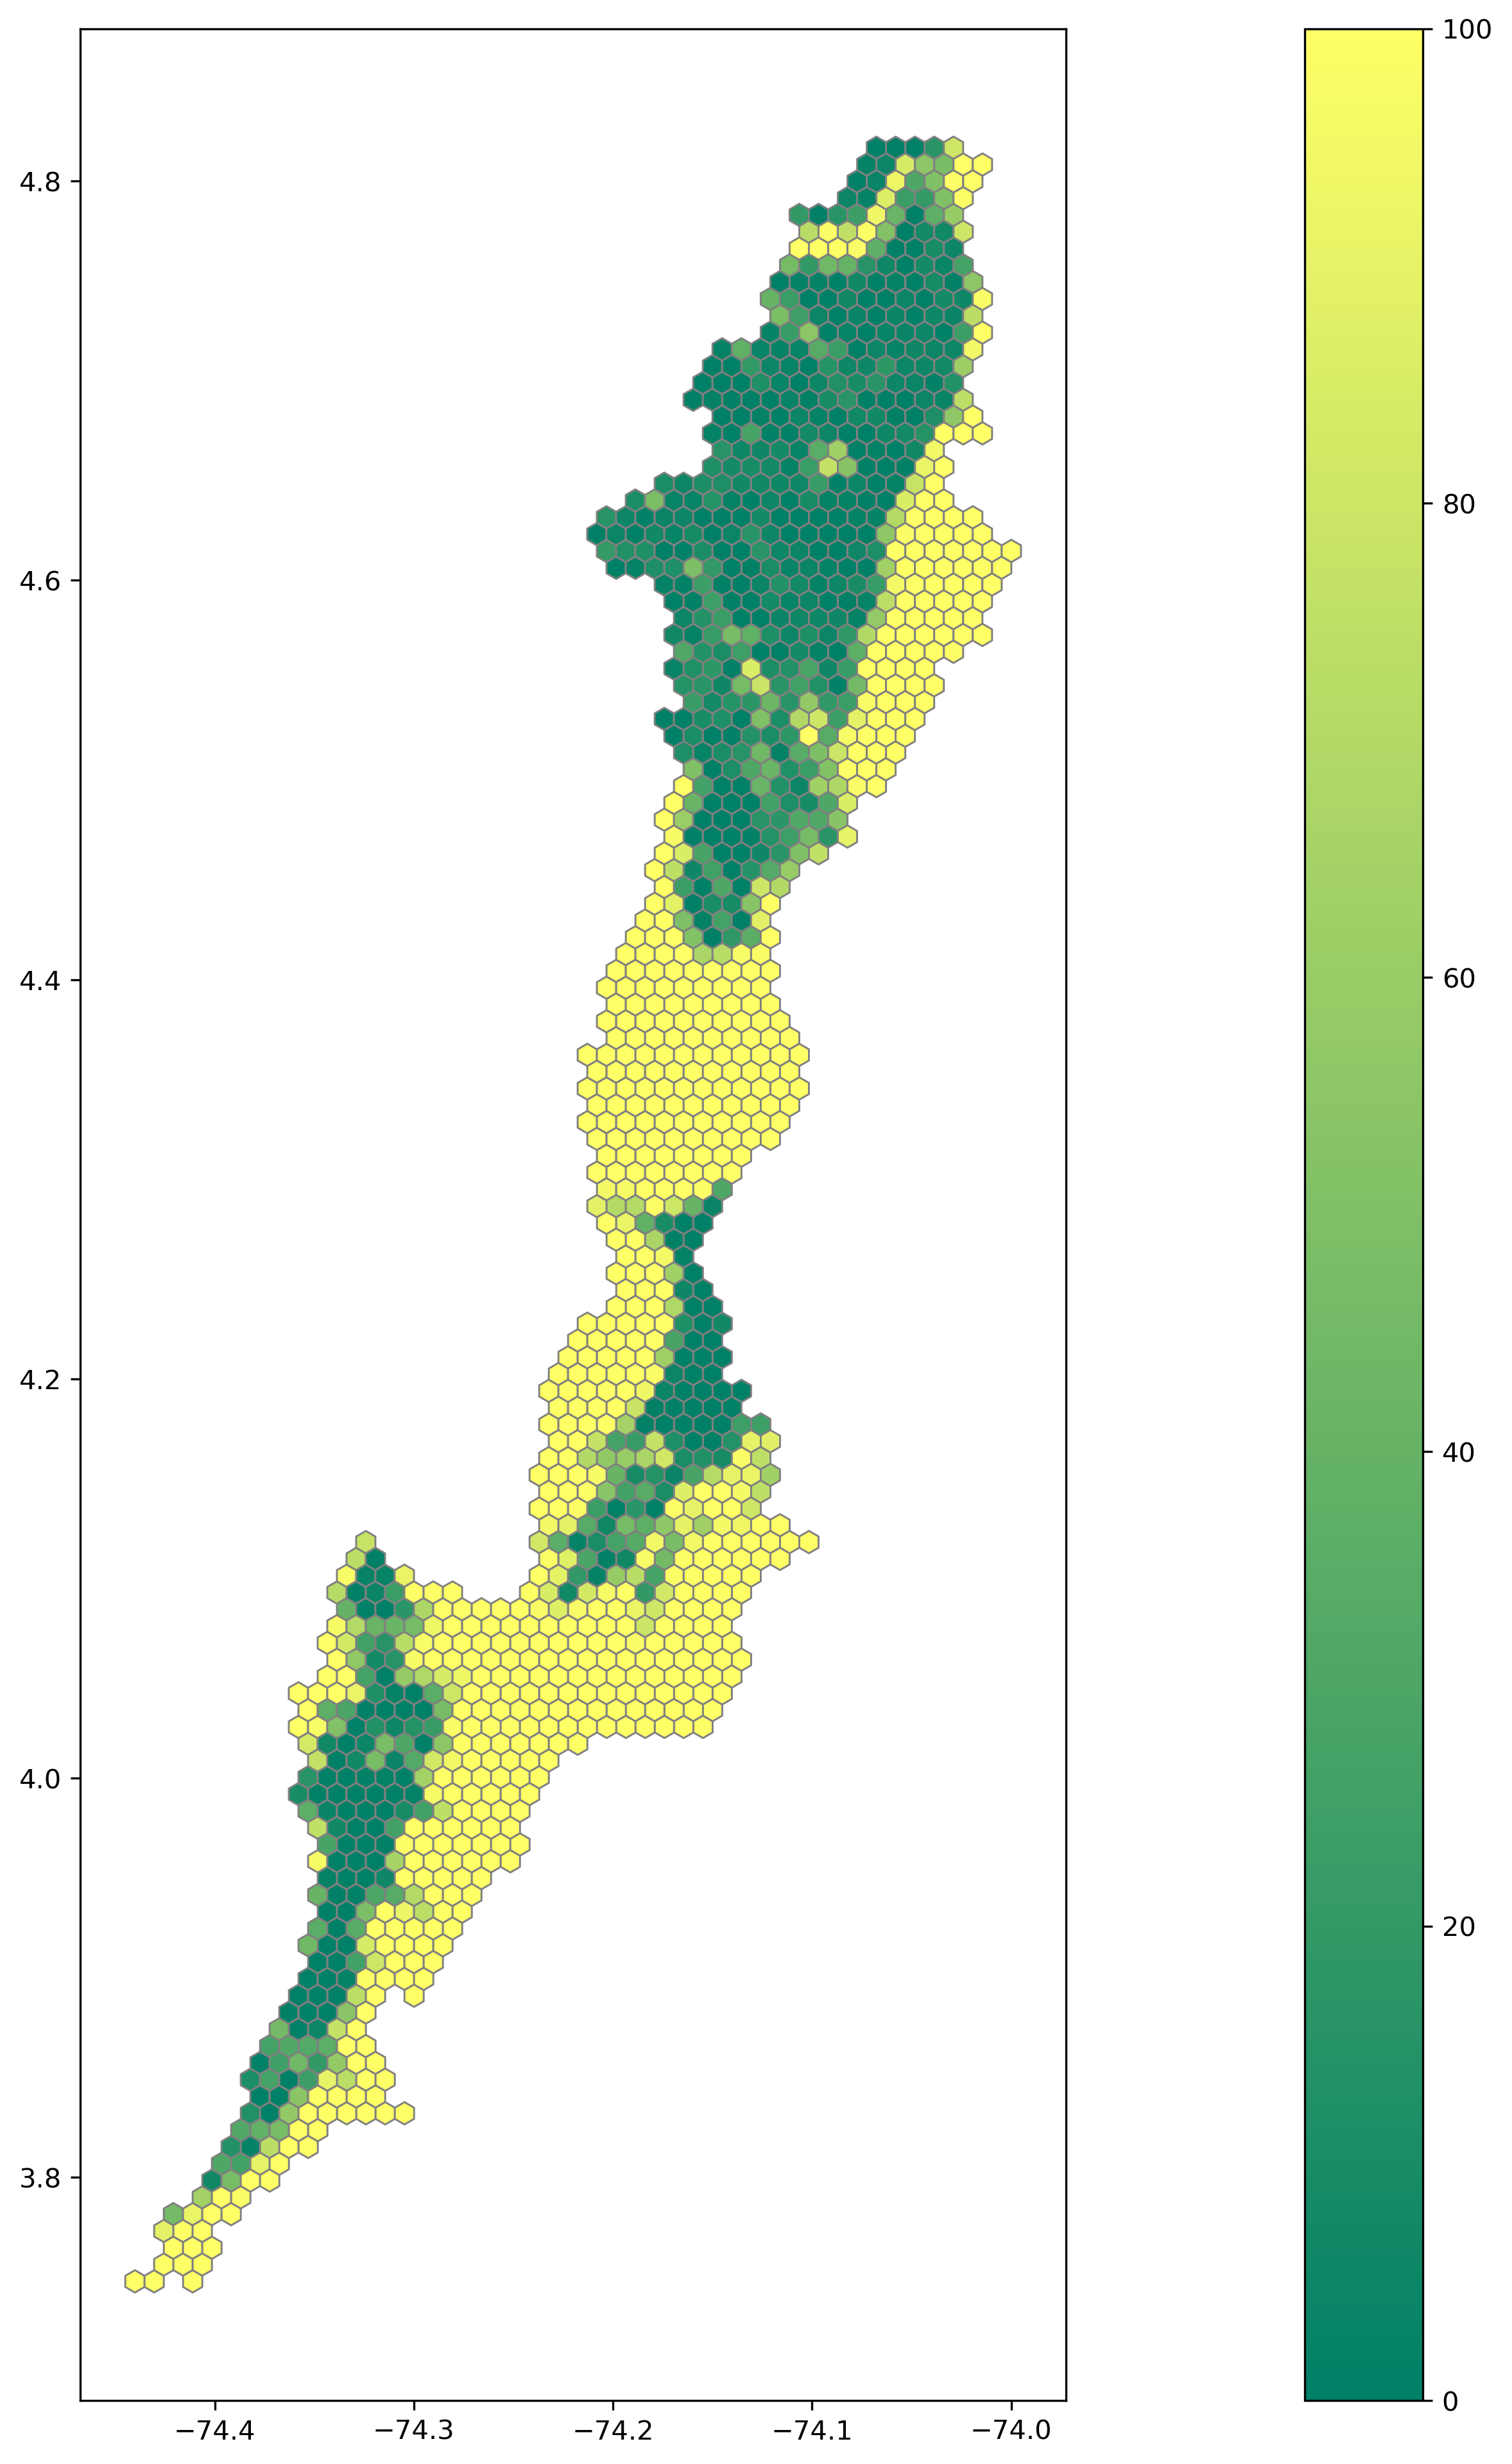
\includegraphics[height=0.8\textheight]{2_conectividad/fig_6.png}
\caption{Mapa de conectividad en las áreas verdes de Bogotá.}
\label{2_conectividad_fig_6}
\end{figure}

\clearpage

\newpage

\section*{Flora de Bogotá}

\noindent \textbf{\large Nelson R. Salinas, Dana S. González y Carlos Vargas}

\noindent \emph{Jardín Botánico de Bogotá, eje Conservación \emph{in situ}}

\bigskip

			
Bogotá cuenta con una gran variedad de paisajes y ecosistemas de la zona alto-andina, lo cual le ha permitido albergar 3181 especies de plantas vasculares, 108 de las cuales se encuentran categorizadas como amenazadas. Aunque la red urbana de parques alberga una gran cantidad de especies exóticas, foráneas del altiplano cundiboyacense, la mayoría de las especies de plantas vasculares bogotanas crecen naturalmente en ecosistemas nativos, como lo son los páramos, los bosques altoandinos y los enclaves secos.

De esta manera, la flora bogotana está dominada por plantas propias de dichos ecosistemas, como lo son las familias botánicas de las compuestas (el grupo de los frailejones, girasoles, manzanillas y caléndula), orquídeas, pastos y leguminosas (el grupo del fríjol, lenteja y arveja). Algunos géneros botánicos son igualmente importantes para la ciudad dada su gran riqueza de especies, como \textit{Epidendrum} (orquídea), \textit{Elaphoglossum} (helecho), \textit{Salvia} (labiada) y \textit{Solanum} (solanácea).

Tradicionalmente, los estudiosos de la flora han enfocado sus esfuerzos en la flora de los cerros orientales. Por esta razón, la flora de los cerros es la mejor conocida y muestreada. Este artificio de muestreo también nos permite entender por qué Monserrate y alrededores registran la mayor riqueza de especies en la ciudad. Sin embargo, en años recientes los botánicos han explorado otras zonas de Bogotá con ávido interés, cubriendo zonas tan remotas como el Parque Nacional Natural Sumapaz y las áreas rurales de las localidades Ciudad Bolívar y Usme, de gran importancia ambiental por sus extensos páramos. En este sentido, es necesario continuar con la exploración botánica de la zona rural de la ciudad, que es donde se han encontrado los vacíos de conocimiento más significativos.


\bigskip

\begin{figure}[b]
\centering

\includegraphics[width=0.7\textwidth]{3_flora/fig_1.pdf}
\caption{Origen de las plantas de Bogotá.}
\label{3_flora_fig_1}
\end{figure}

\begin{figure}[b]
\centering

\includegraphics[width=0.7\textwidth]{3_flora/fig_2.pdf}
\caption{Plantas amenazadas de Bogotá y su categoría en la lista roja}
\label{3_flora_fig_2}
\end{figure}

\begin{figure}[b]
\centering

\includegraphics[width=0.7\textwidth]{3_flora/fig_3.pdf}
\caption{Familias botánicas más diversas en Bogotá}
\label{3_flora_fig_3}
\end{figure}

\begin{figure}[b]
\centering

\includegraphics[width=0.7\textwidth]{3_flora/fig_4.pdf}
\caption{Géneros botánicos más diversos en Bogotá.}
\label{3_flora_fig_4}
\end{figure}

\begin{figure}[b]
\centering
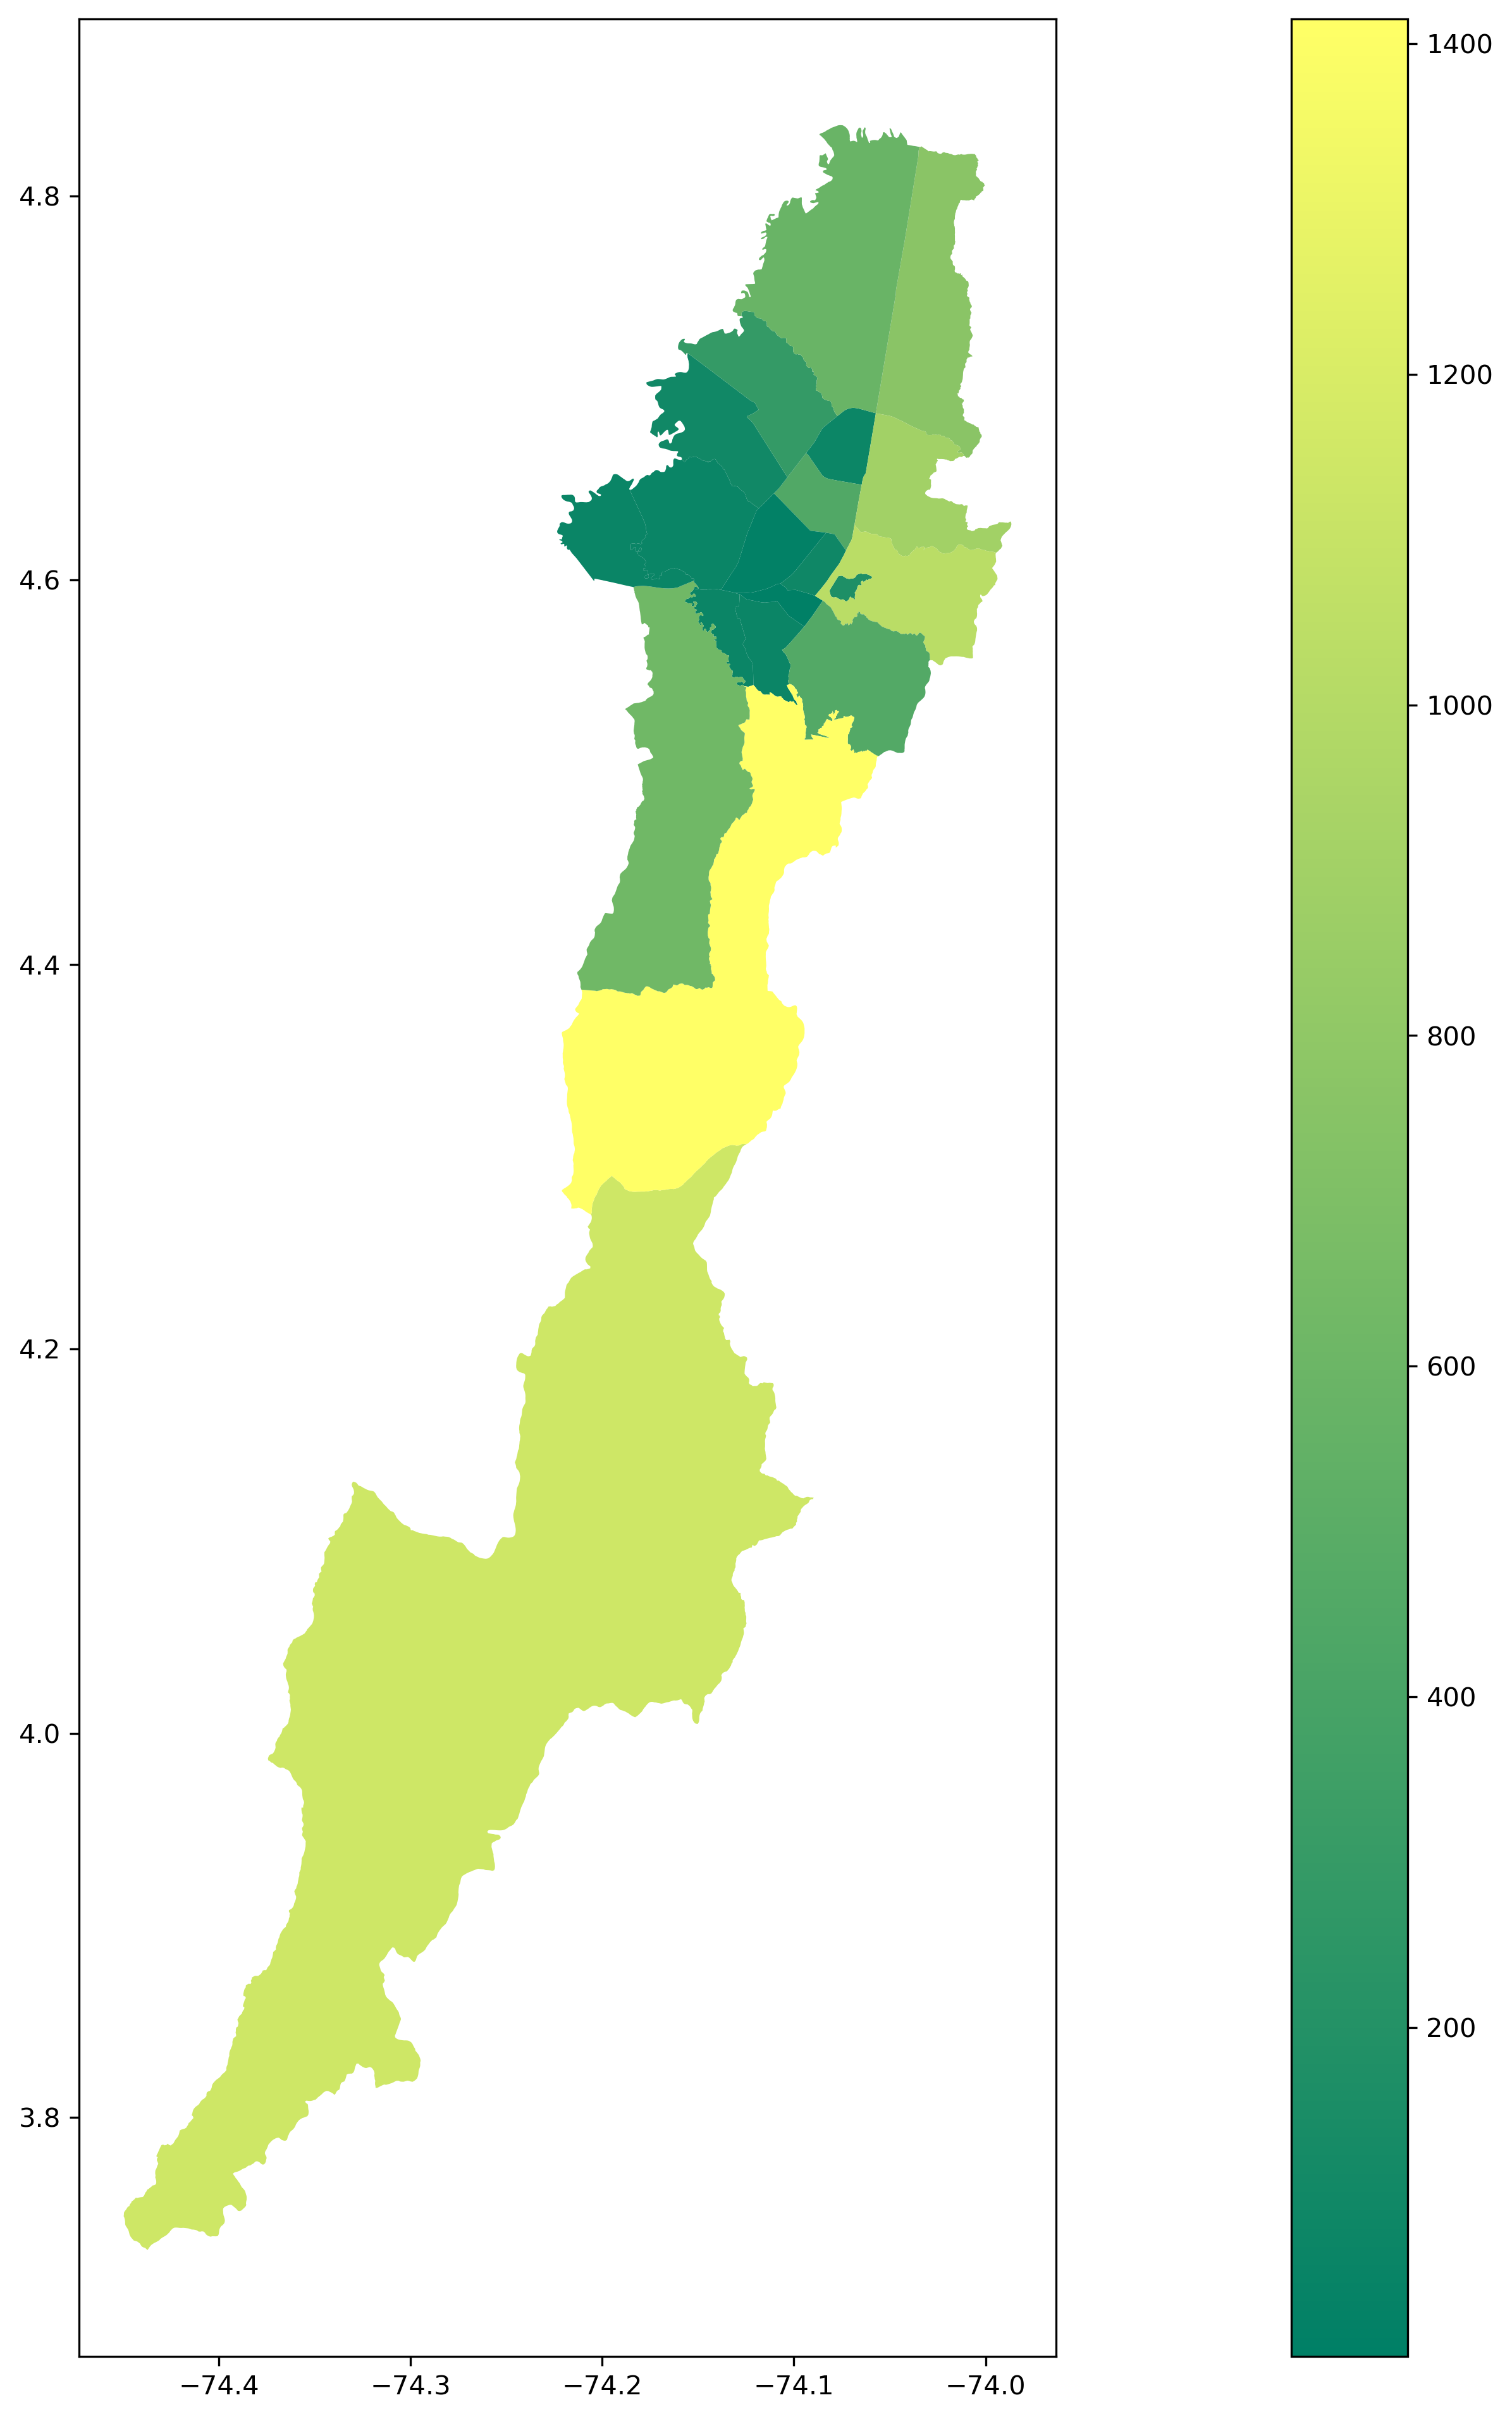
\includegraphics[height=0.8\textheight]{3_flora/fig_5.png}
\caption{Mapa de localidades de Bogotá y su riqueza de plantas}
\label{3_flora_fig_5}
\end{figure}

\clearpage

\newpage

\section*{Plantas de los ecosistemas urbanos y peri-urbanos de Bogotá}

\noindent \textbf{\large Esther Velásquez, Lina Corrales y José Guerrero}

\noindent \emph{Jardín Botánico de Bogotá, eje Conservación \emph{in situ}}

\bigskip

			
La documentación de la flora de Bogotá ha sido una tarea continua desde el siglo XVIII, cuando la real expedición botánica —liderada por José Celestino Mutis— inició el registro de la riqueza vegetal del territorio. Más de dos siglos después, y pese a los numerosos esfuerzos posteriores de investigación, aún persisten vacíos en el conocimiento sobre la composición y el estado de conservación de la flora en el Distrito Capital. Esta investigación busca aportar a la consolidación de esa información mediante la integración de tres estudios desarrollados en 2025 por el eje Conservación \textit{in situ} del Jardín Botánico de Bogotá: la flora de enclaves subxerofíticos andinos, la flora de humedales urbanos y la flora de parques urbanos. 
			
El objetivo de este trabajo conjunto fue caracterizar la diversidad vegetal de tres tipos de ecosistemas representativos de la matriz ecológica urbana y periurbana, fortaleciendo la línea base de flora de Bogotá y evidenciando su papel en la conectividad ecológica y la provisión de servicios ecosistémicos. La consolidación de estas investigaciones permitió generar un panorama unificado de la vegetación bogotana, facilitando el análisis comparativo entre ecosistemas y promoviendo la gestión integrada para su conservación.
			
En los enclaves secos andinos se evidenció una flora predominantemente nativa, rica en especies adaptadas a condiciones de aridez, con rasgos morfológicos como suculencia, espinas y crecimiento herbáceo. Estos ecosistemas conservan un conjunto importante de especies endémicas y constituyen refugios azonales de biodiversidad únicos en el paisaje periurbano de Bogotá. Los humedales urbanos, por otro lado, son de composición mixta, donde conviven especies locales y exóticas, reflejando la influencia antrópica sobre estos ecosistemas. A pesar de ello, mantienen un papel esencial en la conectividad ecológica, la regulación hídrica y la provisión de hábitats para la fauna silvestre. En los parques urbanos, la vegetación representa una transición entre lo nativo y las especies foráneas, con una alta representatividad de especies endémicas, destacando su función como corredores ecológicos y espacios de interacción entre la ciudadanía y la biodiversidad. Estos tres ecosistemas albergan numerosas especies en diferentes categorías de amenaza, lo que resalta la necesidad de fortalecer las acciones de restauración ecológica, manejo de la flora nativa y conservación de los ecosistemas.

En conjunto, este primer Reporte de Estado de la Diversidad en plantas de los ecosistemas urbanos y periurbanos de Bogotá evidencia la alta riqueza florística de la ciudad y la necesidad de continuar unificando datos y esfuerzos interinstitucionales para cerrar vacíos de información, promover la investigación aplicada y consolidar una gestión urbana más resiliente frente al cambio climático.


\bigskip

\begin{figure}[b]
\centering

\includegraphics[width=0.7\textwidth]{4_ecosistemas_urbanos/fig_1.pdf}
\caption{Origen geográfico de las plantas de enclaves subxerofíticos}
\label{4_ecosistemas_urbanos_fig_1}
\end{figure}

\begin{figure}[b]
\centering

\includegraphics[width=0.7\textwidth]{4_ecosistemas_urbanos/fig_2.pdf}
\caption{Origen geográfico de las plantas de humedales}
\label{4_ecosistemas_urbanos_fig_2}
\end{figure}

\begin{figure}[b]
\centering

\includegraphics[width=0.7\textwidth]{4_ecosistemas_urbanos/fig_3.pdf}
\caption{Origen geográfico de las plantas de parques urbanos.}
\label{4_ecosistemas_urbanos_fig_3}
\end{figure}

\begin{figure}[b]
\centering

\includegraphics[width=0.7\textwidth]{4_ecosistemas_urbanos/fig_4.pdf}
\caption{Plantas endémicas de Colombia presentas en los ecosistemas urbanos de Bogotá.}
\label{4_ecosistemas_urbanos_fig_4}
\end{figure}

\begin{figure}[b]
\centering

\includegraphics[width=0.7\textwidth]{4_ecosistemas_urbanos/fig_5.pdf}
\caption{Plantas amenazadas de los ecosistemas urbanos de Bogotá.}
\label{4_ecosistemas_urbanos_fig_5}
\end{figure}

\begin{figure}[b]
\centering

\includegraphics[height=0.8\textheight]{4_ecosistemas_urbanos/fig_6.png}
\caption{Distribución de los ecosistemas urbanos en Bogotá}
\label{4_ecosistemas_urbanos_fig_6}
\end{figure}

\clearpage

\newpage

\section*{Avifauna de Bogotá}

\noindent \textbf{\large Juliana Zuluaga-Carrero}

\noindent \emph{Jardín Botánico de Bogotá, eje Conservación \emph{in situ}}

\bigskip

			
Bogotá se ubica en la convergencia de ecosistemas de alta montaña formados por procesos geológicos y evolutivos de la cordillera oriental, lo que originó una avifauna única con especies endémicas y de distribución restringida. A pesar de su intensa transformación por el desarrollo urbano, la ciudad aún conserva remanentes de ecosistemas andinos que albergan una alta diversidad de aves, una cifra que alcanza 358 especies de aves. Sin embargo, cerca del 70\% del territorio corresponde a zonas rurales donde persisten hábitats como humedales, cuerpos de agua, bosques andinos y altoandinos, enclaves secos, páramos y agroecosistemas.
			
La mayor parte de las especies registradas en la ciudad son residentes (78\%), seguidas de migratorias boreales (17\%), endémicas (2\%), migratorias australes (1\%) y exóticas establecidas (1\%). Su presencia en ecosistemas urbanos, periurbanos y rurales resalta la importancia de Bogotá como un territorio clave para la conservación de la avifauna altoandina. Según las categorías del Libro Rojo de Aves de Colombia, el 89,16\% de las especies de Bogotá no han sido evaluadas, mientras que el 6,96\% se considera en categoría de preocupación menor (LC), un 1,46\% vulnerables (VU), 1,13\% en peligro (EN), 0,65\% casi amenazadas (NT), 0,49\% en peligro crítico (CR) y 0,16\% con datos deficientes (DD).
			 
Actualmente el Jardín Botánico de Bogotá contribuye a un proyecto sombrilla llamado observatorio de biodiversidad y cambio climático, en el marco del cual hemos estado monitoreando la biodiversidad de la ciudad. El observatorio divide a la ciudad en 513 celdas de 2 \texttimes 2 km, en las cuales se analiza la información existente y también se toman nuevos datos. A la fecha, más del 60\% de la ciudad no cuenta con registros y más del 50\% de la información disponible está concentrada en 10 celdas, ubicadas en sitios el Parque Simón Bolívar, Jardín Botánico, Humedal Córdoba, Humedal Burro y Chisacá que llevan la delantera.

Estos valores reflejan tanto la riqueza de avifauna como la necesidad de fortalecer las acciones de monitoreo y protección de los espacios naturales donde estas aves aún subsisten. Con este reporte queremos resaltar el valor de los ecosistemas presentes en Bogotá, no solo como hábitat de especies emblemáticas y endémicas, sino también como espacios fundamentales para el bienestar humano. Aún tenemos una muy baja representación de la avifauna en enclaves secos, bosque altoandinos, plantaciones forestales, bosques urbanos e, incluso, páramos de la ciudad. Invitamos a la ciudadanía a conocer esta biodiversidad como primer paso para diseñar y fortalecer estrategias de conservación para entender sus requerimientos de conservación y asegurar su permanencia en el tiempo.


\bigskip

\begin{figure}[b]
\centering

\includegraphics[height=0.8\textheight]{5_avifauna/fig_1.png}
\caption{Registros de avifauna por localidad de Bogotá.}
\label{5_avifauna_fig_1}
\end{figure}

\clearpage

\newpage

\section*{Biodiversidad y ciencia participativa}

\noindent \textbf{\large Angela Montoya}

\noindent \emph{Jardín Botánico de Bogotá, eje Conservación \emph{in situ}}

\bigskip

			
La Ciencia Participativa es una estrategia que permite la generación del conocimiento de la biodiversidad mediante la observación y registro de especies en distintos puntos de Bogotá, vinculando a la comunidad en los procesos de investigación y conservación. El Jardín Botánico de Bogotá ha venido implementando dicha estrategia en diferentes puntos de la ciudad, contando con la participación de 42 observadores distribuidos en nueve comunidades: cuatro en etapa de diagnóstico, dos en caracterización y tres en monitoreo.
Esta estrategia ha permitido el registro de 3303 observaciones de fauna (aves y artrópodos) y flora. En total, se han reportado 90 especies de aves, 158 de artrópodos y 248 de flora, de las cuales el 45\% corresponden a especies nativas y el 55\% a no nativas. La localidad con mayor número de observaciones es Usaquén, con 10133, seguida de Teusaquillo (377), Puente Aranda (372) y Kennedy (289). También se registró la presencia de especies migratorias, especialmente en las localidades del sur y centro de la ciudad, como \textit{Piranga rubra} (la más observada con 60 registros), \textit{Buteo platypterus} (41 observaciones) y \textit{Contopus virens} (33 observaciones).  
			
Esta estrategia fomenta la educación ambiental, el reconocimiento de la biodiversidad urbana y la generación de datos científicos colaborativos que fortalecen la gestión ambiental de la ciudad.


\bigskip

\begin{figure}[b]
\centering

\includegraphics[width=0.7\textwidth]{8_biodiversidad_cp/fig_1.pdf}
\caption{Distribución de los grupos ciudadanos por etapa de formación.}
\label{8_biodiversidad_cp_fig_1}
\end{figure}

\begin{figure}[b]
\centering

\includegraphics[width=0.7\textwidth]{8_biodiversidad_cp/fig_2.pdf}
\caption{Distribución de los registros biológicos por grupo biótico.}
\label{8_biodiversidad_cp_fig_2}
\end{figure}

\begin{figure}[b]
\centering

\includegraphics[width=0.7\textwidth]{8_biodiversidad_cp/fig_3.pdf}
\caption{Especies con mayor número de registros.}
\label{8_biodiversidad_cp_fig_3}
\end{figure}


\begin{table}[h]
\centering
\begin{tabular}{lrrrr}
\toprule
Zona de estudio & Número de observadores & Aves residentes & Flora & Artropodos \\
\midrule
Parkway & 6 & 15 & 70 & 55 \\
Sta. Bárbara & 22 & 27 & 110 & 81 \\
La Magdalena & 4 & 8 & 30 & 50 \\
Ciudad Montes & 10 & 38 & 60 & 58 \\
\bottomrule
\end{tabular}
\caption[Sitios de trabajo]{Sitios de trabajo en ciencia participativa y principales cifras de biodiversidad registradas por la comunidad.}
\label{bcp_tab}
\end{table}


\clearpage

\newpage

\section*{Interacciones bióticas}

\noindent \textbf{\large Juan Camilo Garibello, Angela Montoya, Esteban Tulande y Juliana Zuluaga}

\noindent \emph{Jardín Botánico de Bogotá, eje Conservación \emph{in situ}}

\bigskip

			
Las interacciones planta-animal son relaciones ecológicas que incluyen mutualismos (como polinización y dispersión de semillas) y antagonismos (herbivoría, depredación), entre otras. Estas interacciones son fundamentales para el funcionamiento de los ecosistemas, la biodiversidad y la evolución de especies, influyendo en la estructura y dinámica de comunidades naturales. Por otro lado, las invasiones de especies exóticas provocan una reducción significativa de la biodiversidad nativa, alterando la composición y estructura de comunidades vegetales y animales. Además, afectan servicios ecosistémicos clave, como la provisión de alimentos, la regulación de la erosión y la polinización, comprometiendo el bienestar humano. La capacidad de las plantas exóticas invasoras para interactuar con la fauna del ecosistema receptor puede influir en el éxito o no de la invasión. Sin embargo, este aspecto ha sido menos estudiado en comparación con otros factores como la competencia con plantas nativas, la abundante producción de semillas y la explotación eficiente de recursos. En Bogotá, las plantas invasoras (tanto nativas como exóticas) mantienen interacciones con la biota local. No obstante, las interacciones de plantas invasoras dentro del grupo de especies foráneas son más comunes: alcanzan el 20\% de los registros de visitas florales y herbivoría, y el 34\% de los registros de epibiosis (colonización de la superficie de la planta por parte de otros organismos como musgos y líquenes , Figura 1). Los registros que involucraron plantas invasoras dentro del grupo de nativas no superaron el 7\% al examinar las mismas interacciones (Figura 2). Cuatro plantas con estatus invasor según "Global Invasive Species Data Base" (GISD) aparecieron entre las 10 especies más registradas en el grupo de exóticas: la palma \textit{Phoenix canariensis} (primer puesto), el árbol \textit{Pittosporum undulatum} (séptima) y las hierbas \textit{Taraxacum officinale} e \textit{Hypochaeris radicata} (cuarta y décima, respectivamente) (Figura 3). \textit{Pittosporum}, una planta ampliamente cultivada a lo largo y ancho de la ciudad, es de particular preocupación dado que se han reportado invasiones de esta especie en bosques montanos tropicales. La literatura reporta efectos ecológicos tanto negativos como positivos de las interacciones de plantas invasoras con biota del ecosistema residente, sin importar si se trata de relaciones en principio mutualistas o en principio antagónicas. La oferta floral de plantas invasoras puede beneficiar polinizadores nativos o la oferta alimenticia de sus hojas puede aumentar la abundancia de insectos invasores a expensas de plantas e insectos nativos. Por lo anterior, es necesario estudiar este tipo de interacciones a mayor profundidad con el fin de entender las invasiones y diseñar, probar y validar alternativas de control.


\bigskip

\begin{figure}[b]
\centering

\includegraphics[width=0.7\textwidth]{9_interacciones/fig_1.pdf}
\caption{Interacciones bióticas de plantas no nativas.}
\label{9_interacciones_fig_1}
\end{figure}

\begin{figure}[b]
\centering

\includegraphics[width=0.7\textwidth]{9_interacciones/fig_2.pdf}
\caption{Interacciones bióticas de plantas nativas.}
\label{9_interacciones_fig_2}
\end{figure}

\begin{figure}[b]
\centering

\includegraphics[width=0.7\textwidth]{9_interacciones/fig_3.pdf}
\caption{Especies no nativas con mayor número de registros.}
\label{9_interacciones_fig_3}
\end{figure}

\begin{figure}[b]
\centering

\includegraphics[width=0.7\textwidth]{9_interacciones/fig_4.pdf}
\caption{Especies nativas con mayor número de registros.}
\label{9_interacciones_fig_4}
\end{figure}

\begin{figure}[b]
\centering

\includegraphics[height=0.8\textheight]{9_interacciones/fig_5.png}
\caption{Mapa de resgistros de interacciones bíoticas por localidad.}
\label{9_interacciones_fig_5}
\end{figure}

\clearpage

\newpage

\section*{Interacciones y ciencia participativa}

\noindent \textbf{\large Angela Montoya}

\noindent \emph{Jardín Botánico de Bogotá, eje Conservación \emph{in situ}}

\bigskip

			
La estrategia Ciencia Participativa e Interacciones Bióticas integra observaciones ciudadanas para caracterizar las relaciones entre organismos que hacen parte de los ecosistemas de Bogotá. A partir de 377 reportes ciudadanos se documentaron diversos tipos de interacción, de los cuales el 72\% corresponde a relaciones de consumo, el 16\% a crecimiento sobre otras especies y un 9\% a interacciones generales, mientras que anidación, parasitismo y simbiosis representaron proporciones menores. El análisis de los recursos consumidos muestra una dominancia del uso de flores (63,8\%), seguida por tallos (11\%), néctar (9,4\%), frutos (7,1\%), hojas y semillas (2,8\% cada una), y polen (1,4\%). Estas interacciones evidencian patrones tanto mutualistas como antagonistas, como \textit{Thygare aethlops} en \textit{Salvia bogotensis}, \textit{Spinus psaltria} en \textit{Streptosolen jamesonii} y \textit{Danaus plexippus} en \textit{Lantana camara}. La información recolectada permite identificar redes tróficas y asociaciones ecológicas relevantes para la gestión de la biodiversidad urbana, aportando a la comprensión de las dinámicas de las especies y la adaptación al desarrollo de la ciudad. El enfoque participativo fortalece la capacidad de observación comunitaria y genera datos verificables para análisis y seguimiento de dinámicas biológicas en el Distrito Capital.


\bigskip

\begin{figure}[b]
\centering
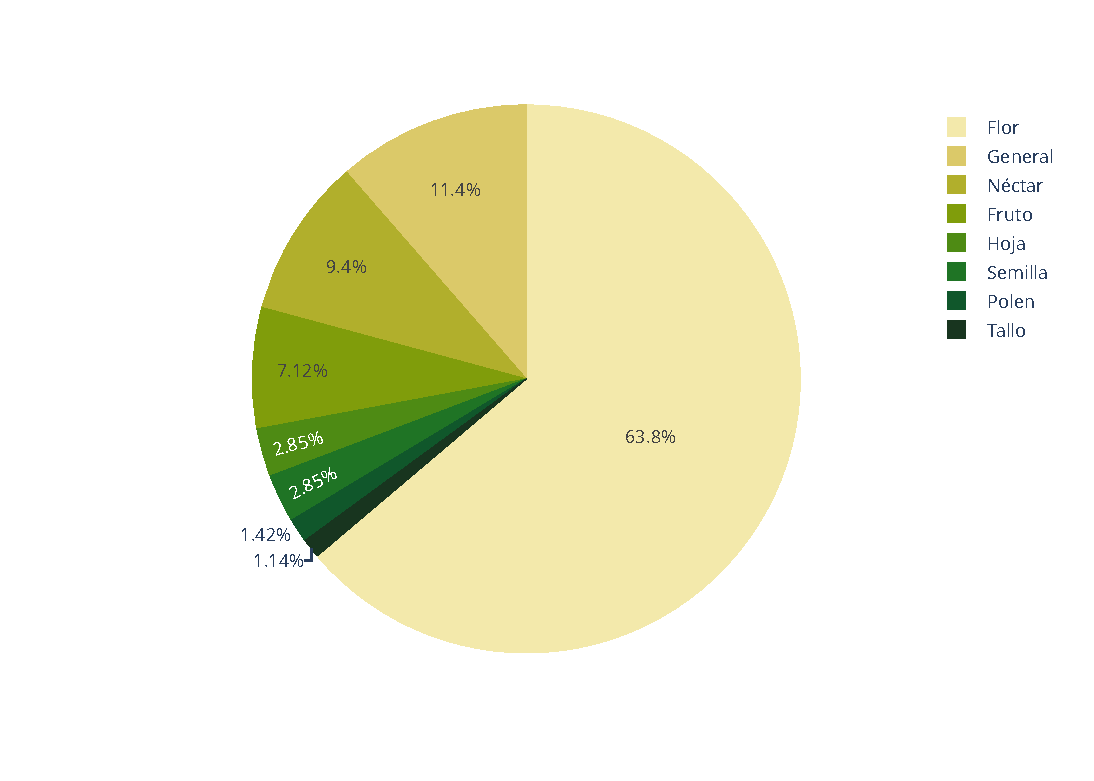
\includegraphics[width=0.7\textwidth]{10_interacciones_cp/fig_1.pdf}
\caption{Recursos bióticos asociados a registros de interacciones.}
\label{10_interacciones_cp_fig_1}
\end{figure}

\begin{figure}[b]
\centering
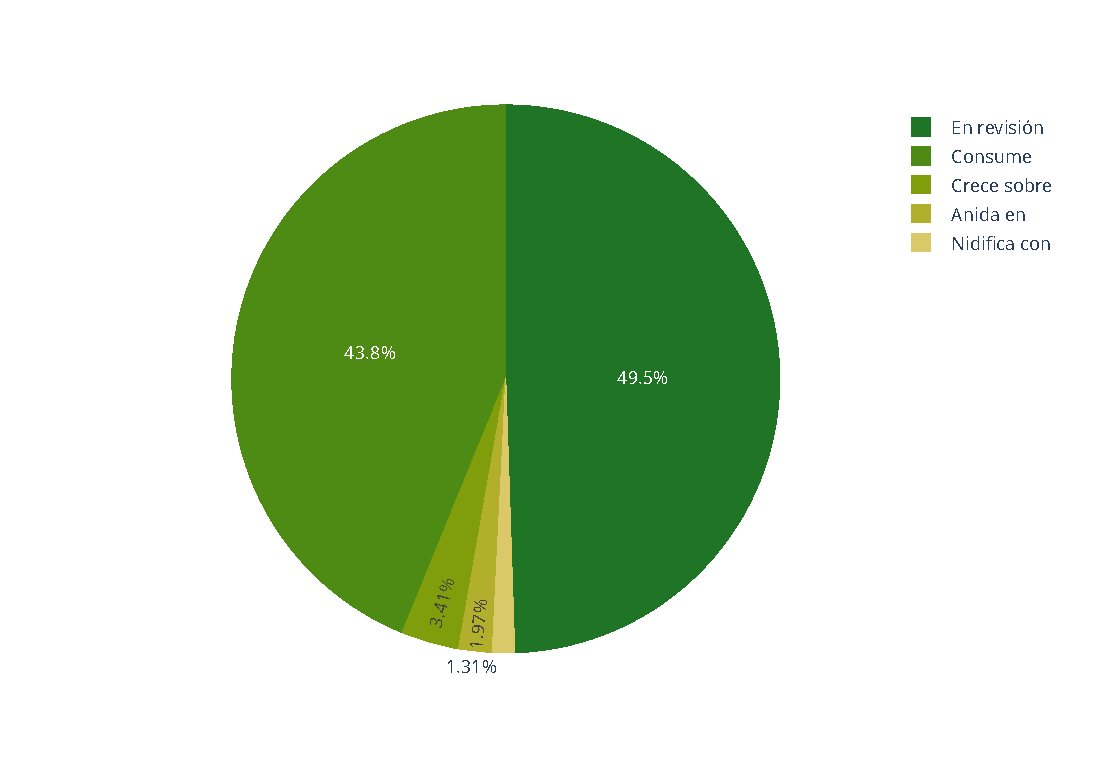
\includegraphics[width=0.7\textwidth]{10_interacciones_cp/fig_2.pdf}
\caption{Clases de interacciones registradas.}
\label{10_interacciones_cp_fig_2}
\end{figure}

\clearpage

\newpage

\section*{Hojarasca y suelos en áreas de importancia ecológica de Bogotá}

\noindent \textbf{\large Angie Montañez y Luisa Betancourt}

\noindent \emph{Jardín Botánico de Bogotá, eje Conservación \emph{in situ}}

\bigskip

			
En áreas verdes urbanas, el suelo además de ser un refugio de biodiversidad es un aliado estratégico para la mitigación del cambio climático. En este estudio se analizó la variación del aporte de hojarasca fina, el flujo de CO\textsubscript{2} y algunas propiedades del suelo (carbono, materia orgánica, pH y densidad aparente) en tres áreas de importancia ecológica de Bogotá (El Jardín Botánico de Bogotá, Las Mercedes y el Bosque Urbano de Ciudad Montes - BUCM). El Jardín Botánico exhibió un mayor aporte de hojarasca (4.17 t ha\textsuperscript{-1}) y flujo de CO\textsubscript{2} (2.77 µmol m\textsuperscript{-2} s\textsuperscript{-1}), lo que sugiere mejor actividad biológica y respiratoria en el suelo. En las Mercedes se presentaron valores intermedios de hojarasca y CO\textsubscript{2} del suelo; mientras que el BUCM presentó los valores más bajos en aporte de hojarasca (1.49 t ha\textsuperscript{-1}) y flujo de CO\textsubscript{2} (1.56 µmol m\textsuperscript{-2} s\textsuperscript{-1}). En relación con las propiedades del suelo, el BUCM exhibió un valor alto de carbono orgánico (180.2 t ha\textsuperscript{-1}), sugiriendo un alto potencial de secuestro de carbono pese a que la densidad aparente refleja compactación y baja aireación del suelo. Estos hallazgos evidencian que las áreas verdes urbanas pueden actuar como sumideros de carbono, especialmente cuando se implementan prácticas de conservación del suelo, como mantener la cobertura de hojarasca.


\bigskip

\begin{figure}[b]
\centering

\includegraphics[width=0.7\textwidth]{11_suelos/fig_1.pdf}
\caption{Composición de la hojarasca.}
\label{11_suelos_fig_1}
\end{figure}

\begin{figure}[b]
\centering

\includegraphics[width=0.7\textwidth]{11_suelos/fig_2.pdf}
\caption{Flujo de gas carbónico en el suelo.}
\label{11_suelos_fig_2}
\end{figure}

\begin{figure}[b]
\centering
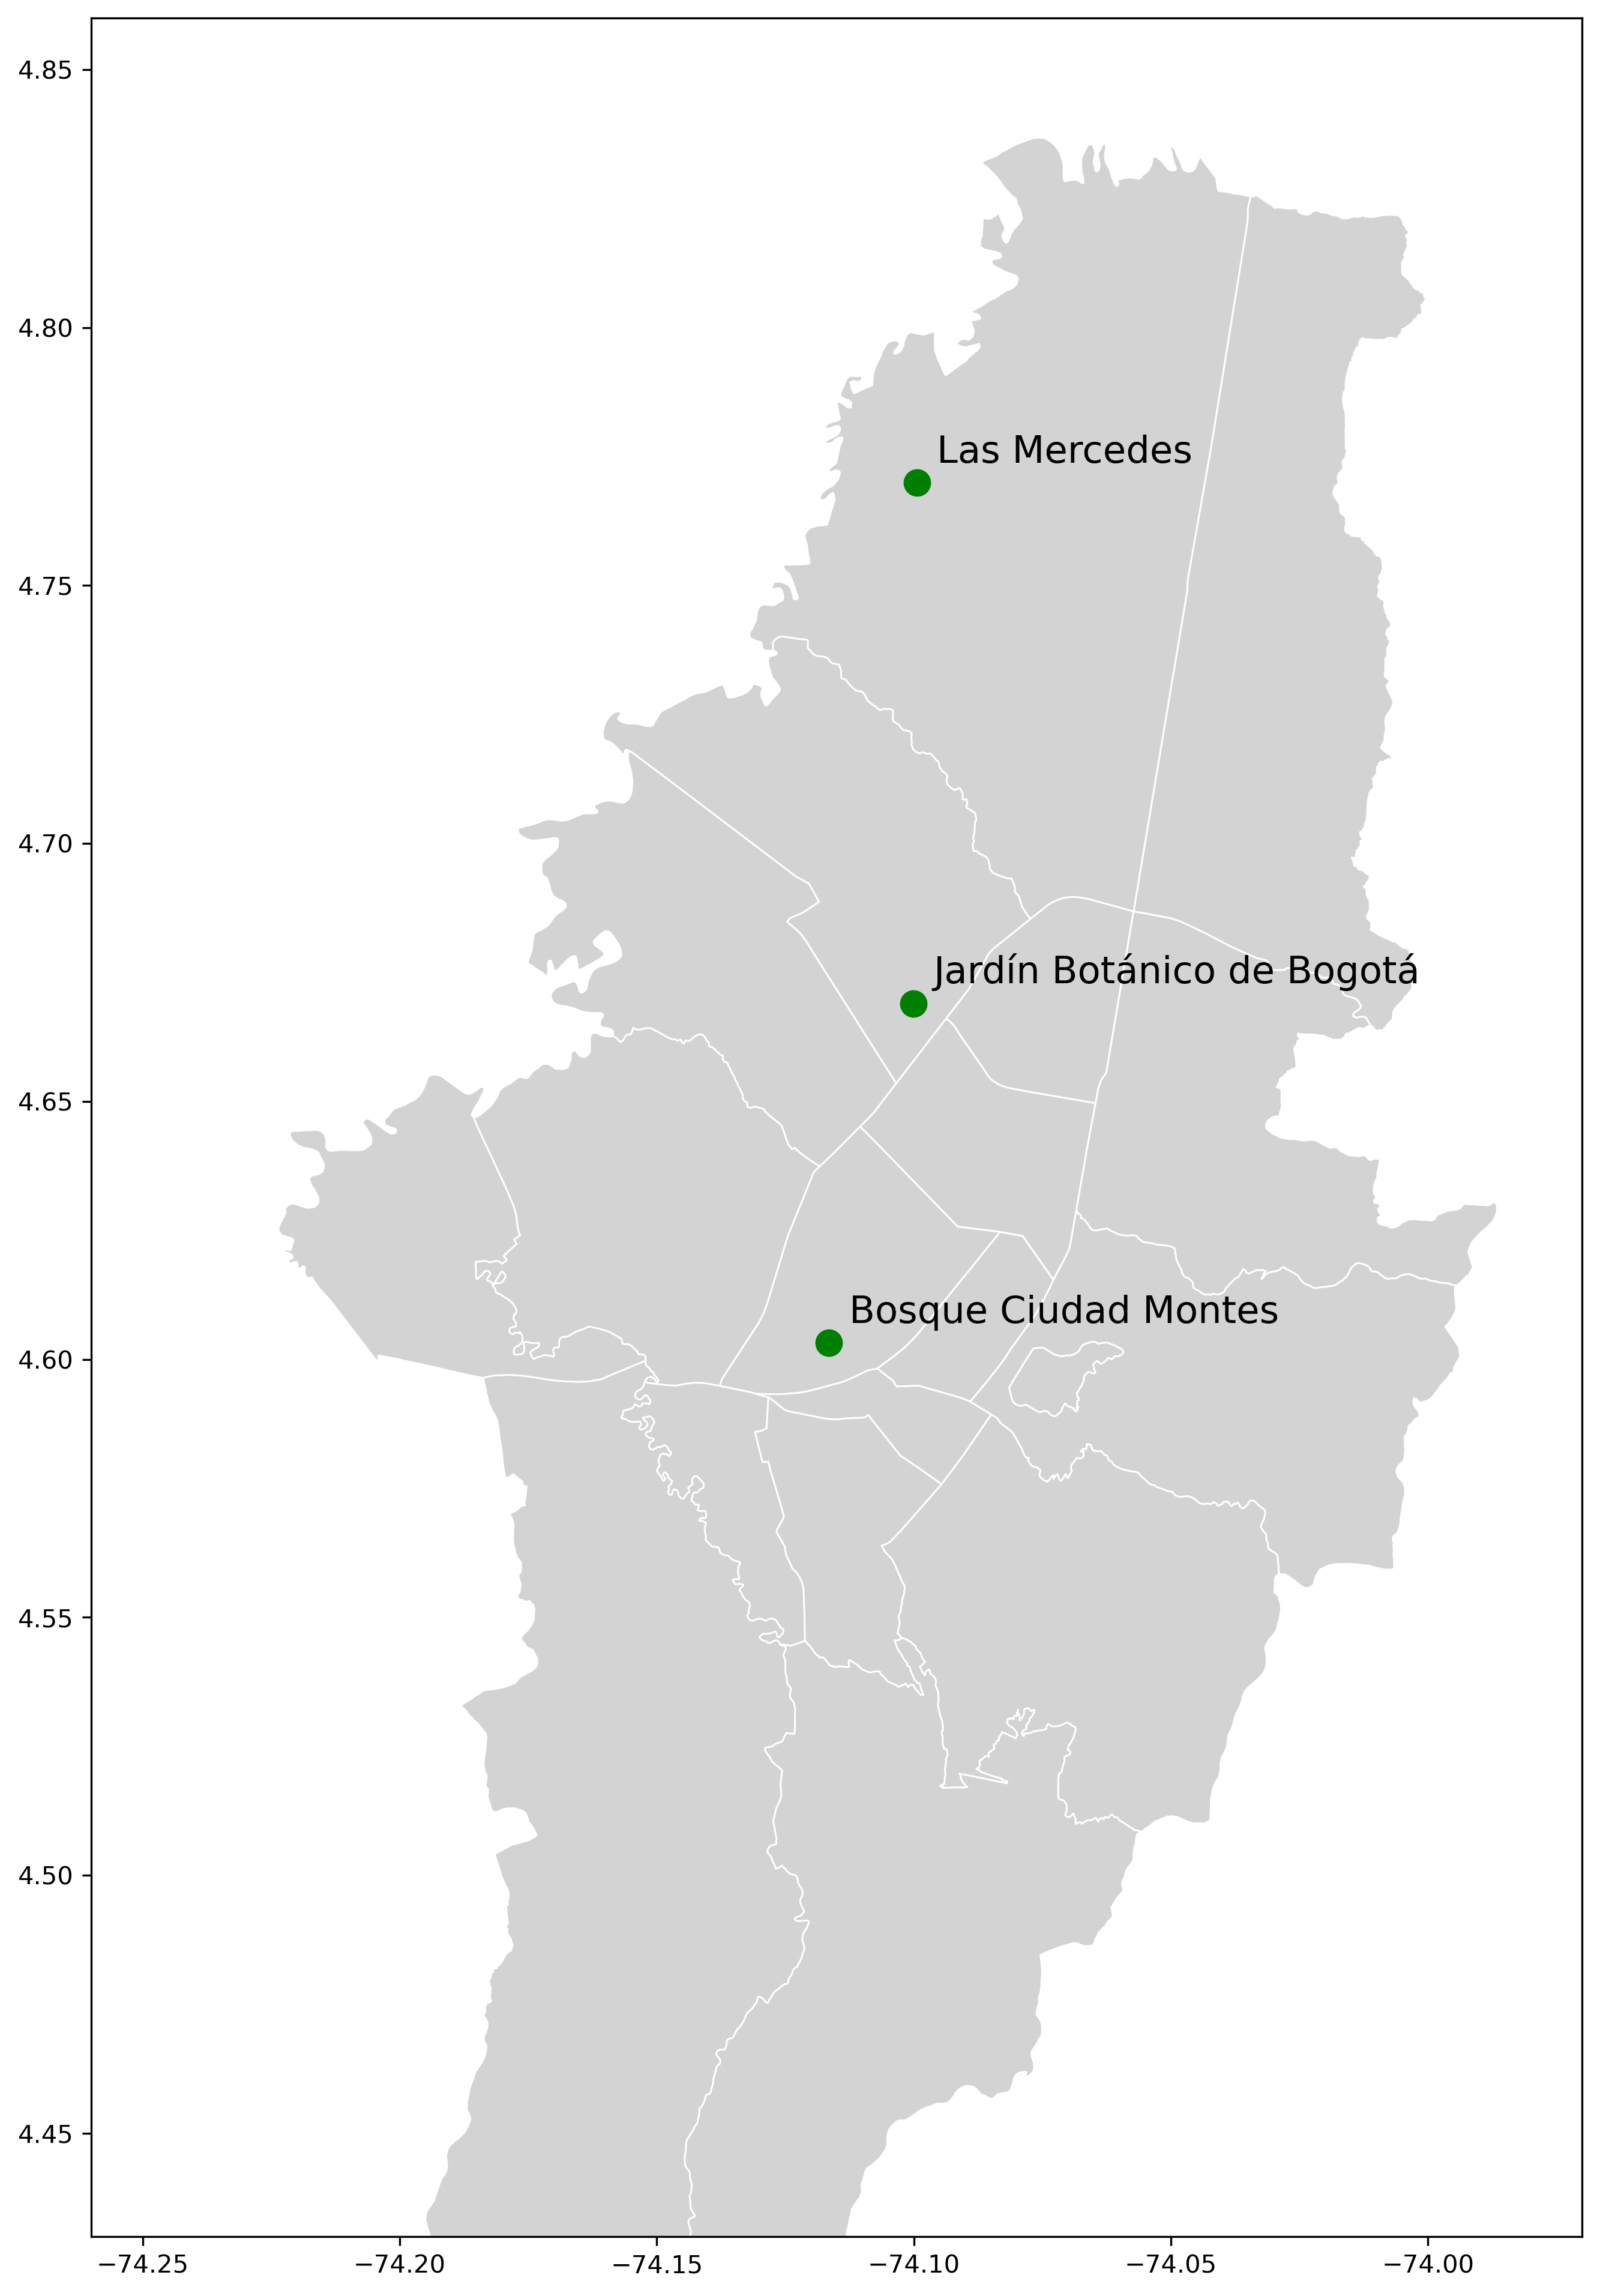
\includegraphics[height=0.8\textheight]{11_suelos/fig_3.png}
\caption{Lugares de trabajo durante la vigencia 2025.}
\label{11_suelos_fig_3}
\end{figure}


\begin{table}[h]
	\centering
\begin{tabular}{lrrr}
\toprule
Característica & JBB & MER & BCM \\
\midrule
Materia orgánica (\%) & 23.900000 & 32.000000 & 17.500000 \\
Carbono orgánico (\%) & 13.900000 & 18.600000 & 10.200000 \\
Densidad aparente (g cm\textsuperscript{-3}) & 0.780000 & 0.590000 & 1.000000 \\
pH & 5.810000 & 5.820000 & 6.210000 \\
Carbono (t C ha\textsuperscript{-1}) & 128.800000 & 203.200000 & 180.200000 \\
\bottomrule
\end{tabular}
\caption[Variables fisico-químicas]{Principales variables fisico-químicas de los suelos estudiados. JBB: Jardín Botánico de Bogotá, MER: Las Mercedes, BCM: Ciudad Montes.}
\label{sue_tab}
\end{table}


\clearpage

\newpage

\end{document}

